\section{Control layer}

%layer overview
This layer is responsible of connecting the physical and the logical layers of the system, connecting the physical variations that produce the signal with the logical information they carry.
For a transmitter this translates to the process of producing variations of the physical properties in a structured way according to what dictated by the logical layer, in a way that these variations reflect the information given.
For the receiver, the control layer is responsible of reading the values from the sensory layer and forward them to the logical layer, perform filtering and other minor operations.
In the prototyped system, this layer is physically represented by micro controller boards connected with a terminal through a serial connection on one side, and with the components of the physical layer on the other.
This layer is crucial for establishing performance of the system in terms of \textbf{rates}, as in how many values can be read from a sensor per time unit for reception, and how fast can a signal be sent to control the light emitter for transmission.

%serial connection
\subsection{Connection to the logical layer}
Being in the middle of the system, this layer has two connections, one outgoing and one incoming.
The transmitter will have an incoming connection with the logical layer and one outgoing to the physical, while the receiver will have an outgoing connection to the logical layer and one incoming from the physical layer.
Since this layer is the one that produces transmission and reception rates, it's worthwhile to spend some time in analysing both types of connections, because the sum of both will result in the overall performance of this layer.
Transmission rate, as will be discussed, depends on the speed of the outgoing connection from control layer to the physical layer for obvious reasons.
However, the speed of the incoming connection from the logical layer would also play a role.
The same discussion applies for the reception rates, in reverse.
In the prototype, the connections between control and logical layer are implemented as serial connections between the controller board and the terminal where the logical layer is running.
Both boards are Arduinos, and handle the serial connection in the same way.
There are a few aspects to consider when implementing the link between control layer and logical layer, from the logical layer point of view.
One aspect to consider is that the serial buffer has a limited size of 64 bytes in most Arduino boards, so it's important to keep the serial communication as light as possible to avoid overflow and loss of information.
This means that if the message that needs to pass through is encoded as a string, it would need to be sent one character at a time and avoid unnecessary additional information.
In most cases, it's possible to encode a single character into one single 8-bits byte, but not all the programming languages implement this automatically.
The system prototyped in this case was implemented using Python 2.7, which uses dynamic types and therefore doesn't have a specific type for \textit{chars}. 
In Python, strings are objects with an overhead of 37 bytes, plus one byte for every character in the string.
This would result in a very heavy serial transmission for just a few characters. Characters need to be converted in single bytes before sending them. 

\todo{information about clock rates of the boards}

%reception
\subsection{Reception rates}
\label{recrates}
Reception happens as fast as the micro controller allows, in fact the control process doesn't force a specific speed on the analog input coming from the sensor, but rather the rate of reception is bound to the clock rate of the processor in the control layer and the speed of the physical sensor.
The average reception rate is of about one value every 0.833 ms, about 1200 Hz (or bits per second).
This value naturally becomes the upper bound for the transmission rate, since if signals were sent faster, they wouldn't be received in time. 
The control layer also performs the two operations of appending a timestamp to each value once received before sending it to the next process, and filtering each value as an average of its direct predecessor and itself, to reduce noise.
With the use of timestamps it's fairly simple to measure the reception rate before the serial connection.
This rate is not constant, but has a standard deviation of about 0,0184 ms.

%transmission
\subsection{Transmission rates}
The transmission process takes as input a message that needs to be converted into Manchester code (see \ref{modulschemes}).
Just like pure binary, Manchester encoding only has two symbols, 1s and 0s.
A symbol, in telecommunication, represents the smallest amount of data that can be sent in form of an analog signal. The symbol rate (symbols per time unit) is measured in baud.
Each pair of symbols in Manchester represent a single binary bit. 
Given the limitations for the reception side, it's in practice very difficult to measure transmission rates above 1000 Hz in the prototype system.
The reception rate imposes a first limitation on the transmission rate, since transmission faster than reception would be extremely faulty.
A second limitation is introduced by the physical speed of the LED used.
From the measurements of warmup times of the LED presented in section \ref{physical}, it's possible to see what amount of variations are achievable in 1 ms, which would result in a rate of 1000 Hz.
In the best case, it's at most a 30\% increase starting from 0 and a 25\% decrease starting from 100, although in average it would be less.
Along the middle of potential brightness, where transmission is supposed to happen, 1 ms could cause a variation of about 15\% in brightness.
The control layer is directly responsible for the transmission rate, therefore it needs to guarantee a rate that allows a reliable reception.
The previous limitations in reception rate and LED speed would suggest that a maximum acceptable rate is of 1000 Hz, with a potential difference between an average 1 and an average 0 of at most 15\% of brightness, and a reception rate that is slightly higher.
Would this rate produce acceptable readings on the receiver side?\\
Experimentally it was found that sending signals at 1ms intervals produces a degree of uncertainty of about 30\%, while a 2 ms interval performs much better at 0\% uncertainty.
More on the experiments and results in section \ref{tr:rate:exp}.
According to these results, each single symbol is forced to last for 2 ms before the transmitter board can send the next.
The transmission rate would therefore be at best of 500 bauds in theory, in the case where the activity of the micro controller pays no role.
This value was experimentally measured to be slightly smaller, at around 450 bauds. 

%experimentations for tx rate
\subsection{Experiments and Results for Transmission Rate}
\label{tr:rate:exp}

To find the perfect transmission rate experimentally, the prototype has been set up to transmit sequences of alternating 1s and 0s of known length multiple times.
For this experiment, the distance and angle from the sensor to the light source have been minimised to obtain the best reception possible.
The experiment aims to measure and count the number of local maximums and local minimums in the transmission, that would define the number of 0 and 1 signals received.
Also, the brightness levels have been measured for such local peaks.\\
The fist transmission rate to be tested is a 1000 bps rate, with an interval of 1 ms between subsequent signals.
Over 30\% of the signals haven't been received.\\
A second rate of about 500 bps has also been tested to compare with the first one.
This time the interval between two subsequent signals is of 2 ms.
Intervals of 3 ms and 4 ms have also been tested.
Table \ref{ratestable} shows the results of various measurements with the various rates, while fig. \ref{fig:txpeak} shows overlapped samples of the transmissions with the different setups.\\
As can be seen in the figure, during transmission the brightness achieved from the LED used for testing is not at 100\%, but transmission is still clearly recognised at a level of about 60\%. 
In the figure, the starting and ending points of the transmission are at the minimum and maximum brightness level of the LED, to the far left and far right respectively.\\
The transmission is always the same over all the instances and in all setups.
Reception of the same message in different rates happens at different speeds, consistently with the rate difference.
The x-axis in the figure shows the progression of time receiving the message, and it appears clear that lower rates produce slower receptions.
Another difference that is clearly noticeable is that the difference between 1s and 0s also varies depending on the time that the signal is forced to stay on.
These results suggest that the lower the rate, the more reliable the communication, since broader variations would be more robust to interference and noise.
However, the rate of 2 ms per signal has been chosen to be final transmission rate in the prototype system with the low power LED, being the fastest reliable rate.
With a system that uses a different light emitter, or designed to be used at longer distances, different experiments would be advised.
\begin{figure}[hbt]
\centering
  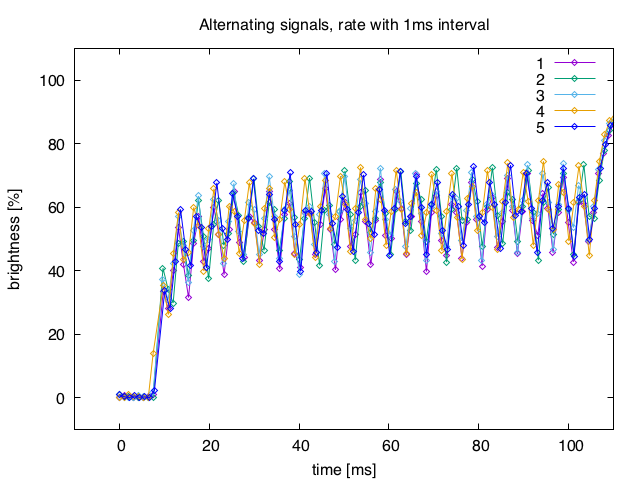
\includegraphics[height=140px]{img/overlap1}
  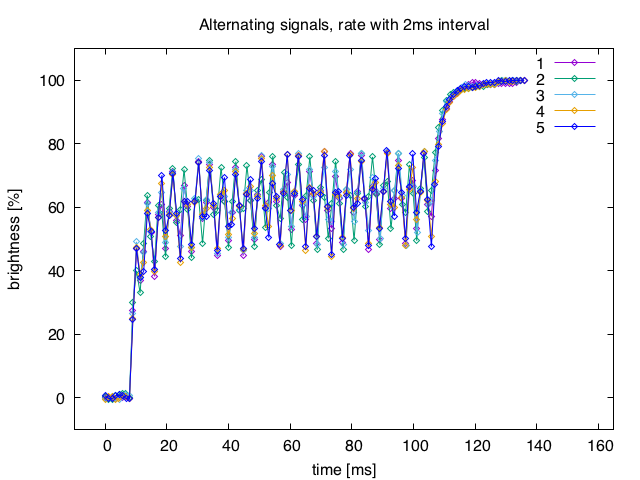
\includegraphics[height=140px]{img/overlap2}
  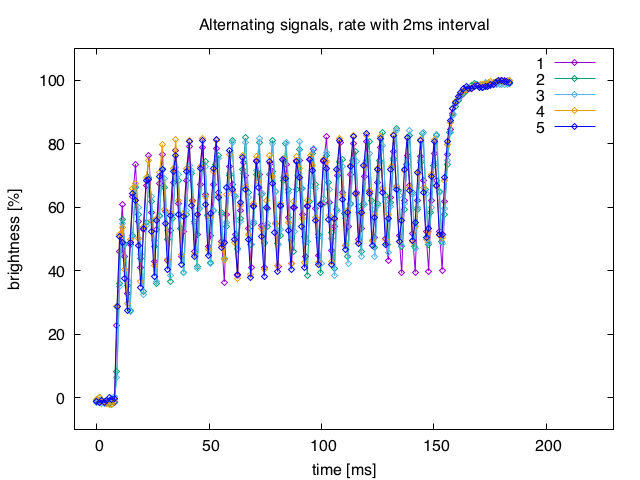
\includegraphics[height=140px]{img/overlap3}
  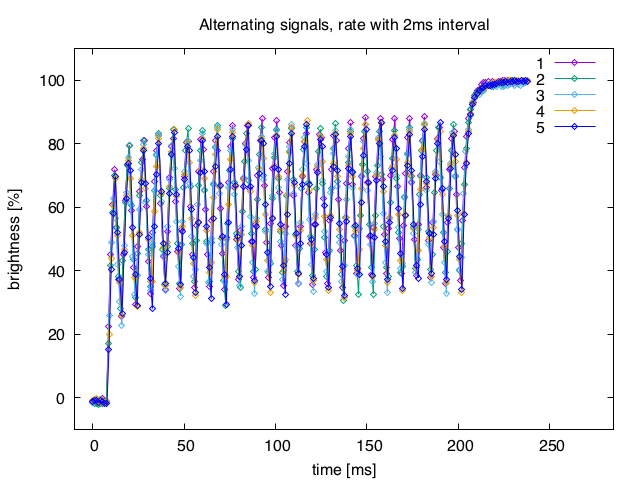
\includegraphics[height=140px]{img/overlap4}
  \caption{Test of rate with 1 ms, 2 ms, 3 ms and 4 ms intervals (left to right, top to bottom).}
  \label{fig:txpeak}
\end{figure}

\begin{table}[hbt]
\centering
 \begin{tabular}{l c c c r}
   rate interval & missing 1s & missing 0s & average 1 brightness & average 0 brightness \\
   \hline
   1 ms & 34.52\% & 30.62\% & 66.75\% +- 6.10 & 55.78\% +- 6.72 \\
   2 ms & 0.00\% & 0.00\% & 70.22\% +- 7.06 & 50.18\% +- 5.79 \\
   3 ms & 0.00\% & 0.00\% & 76.72\% +- 6.18 & 43.03\% +- 5.20 \\
   4 ms & 0.00\% & 0.00\% & 82.77\% +- 4.00 & 35.54\% +- 3.60 \\
   \hline
	\end{tabular}
  \caption{Rates results compared.}
  \label{ratestable}
\end{table}

\begin{figure}
\centering
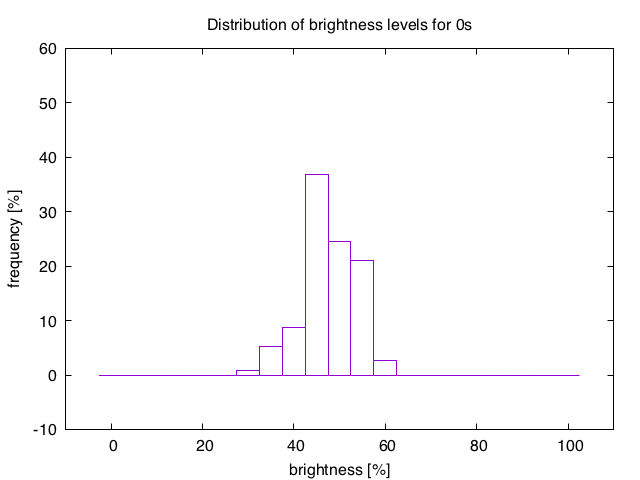
\includegraphics[height=100px]{img/hist0}
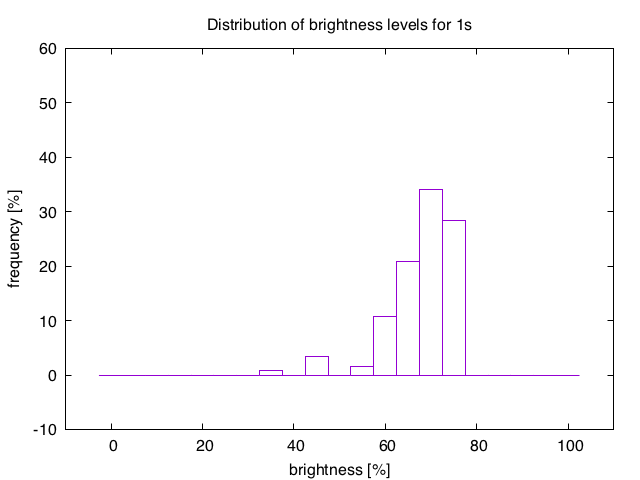
\includegraphics[height=100px]{img/hist1}
\caption{Distributions of brightness levels during transmission (2 ms interval), brightness of binary 0s to the left, 1s to the right. }
\label{fig:histopeaks}
\end{figure}


%distance
\subsection{Distance}
As we can see from table \ref{ratestable}, 2 ms is the fastest reliable rate, but how does it scale over different distances?\\
In section \ref{distancephy} it was discussed how distance influences the reception in terms of maximum brightness registered from the sensor.
However, a new relevant question is how distance would influence reception when there is transmission.
Like in the previous paragraph, an answer to this question can be found experimentally by repeatedly switching the light on and off, and measuring the characteristics of the signal that is received, at different distances.
\begin{table}[hbt]
\centering
  \begin{tabular}{l c c c c c}
    distance & max. brightness & missing 1s & missing 0s & average 1 brightness & average 0 brigthness\\
    \hline
    0cm & 100\% & 0.00\% & 0.00\%  & 70.22\% +- 7.06 & 50.18\% +- 5.79 \\
    10cm & 42.81\% & 0.00\% & 0.00\%  & 60.30\% +- 10.64 & 43.61\% +- 10.67 \\
    20cm & 14.28\% & 4.68\% & 4.68\%  & 49.99\% +- 12.22 & 36.41\% +- 12.01 \\
    30cm & 8.57\% & 2.38\% & 1.78\%  &  54.49\% +- 18.83 & 39.69\% +- 20.37 \\
  \end{tabular}
  \caption{Test of 2ms rate over different distances.}
  \label{tab:2msdistances}
\end{table}

Table \ref{tab:2msdistances} shows the results of these experiments.
Contrarily to section \ref{distancephy}, the percentages of brightness are relative to each separate experiment, in the sense that each separate experiment with a different distance has a different level for 100\% of brightness received.
 This means that for each experiment, a 100\% represents the maximum brightness measured in that experiment.
This is to shift the focus on the variations and the relation between high signals and low signals, to ultimately verify if even at different overall brightness levels transmission is still comparable.
Maximum brightness levels are still reported on the table however.
Two important aspects emerge from these results: one, that reliability remains reasonably high, and two that uncertainty in the average brightness for 1s and 0s grows a lot, probably due to the increasing weight of noise.

% big light
\subsection{Controlling AC powered lights}
\todo{ssr talk}
As was mentioned, the control layer is supposed to control the switching of the light bulb by directly control its power supply.
This is easily achieved in the prototype since the LED is powered directly from the controller board.
However, in the optic of using light bulbs powered from AC mains, the controller layer would need to act differently.
Different switching mechanisms have been tried, and by far the most performant resulted to be a Solid State Relay switcher, or SSR for short.
A SSR has the power to close or open the circuit connected to the AC source. With a small activation signal it can allow the current to flow through or stop it.
The activation signal can easily be sent from the controller board.
However, the use of a SSR brings additional limitations to the system, especially on possible speed achievable in transmission.
Although faster than other types of relays, SSRs still have some limitations, like in the activation speed. 
Fast switching at a rate faster than the activation time of the relay will have no effect, and switching at a rate that is only slightly slower will allow only a limited amount of current through before switching off, as the experiments suggest. \todo{experiments ssr}
\todo{graph of ssr speed (real/bigLED/test1)}
\todo{wiring with ssr diagram}
